\documentclass[12pt,a4paper,utf8]{ppgsi}
\usepackage{epstopdf}
\usepackage{natbib}
\usepackage{multirow}
\usepackage{breqn}
\usepackage{lscape}
\usepackage{amssymb}
\usepackage{algorithm,algorithmic}

\title{Relatório Técnico da disciplina Aprendizado de Máquina}

% Autores, como aparecem na capa do RT
\coverauthor{Renata C. B. Madeo\\ Lucas Brunialti\\ André Barata}

% Autores do documento
\author{Renata C. B. Madeo\inst{1}, Lucas Brunialti\inst{1}, André Barata\inst{1}}

\address{Escola de Artes, Ciências e Humanidades --
    Universidade de São Paulo\\
    São Paulo -- SP, Brasil
    \email{renata.si@usp.br,lucas.brunialti@usp.br,andre.barata@usp.br}
}

% Número do RT
\numero{001/2014}

% Mês e ano do RT
\mes{08}
\ano{2014}

\begin{document}

\maketitle

\begin{abstract}

Devido à alta procura e o alto grau de risco que o investimento em ações proporciona, muitos procuram por métodos para prever tendências do valor das ações. Este trabalho tem como objetivo prever a tendência do fechamento do Ibovespa em alta, baixa ou estável, a partir do histórico do próprio índice e dos índices de bolsa de valores da América, Ásia e Europa fazendo uso de técnicas de Aprendizado de Máquina. Para atingir este resultado foram utilizadas técnicas baseadas em Aprendizado de Máquina: Regressão Logística, Rede Neural Multilayer Perceptron, \textit{Extreme Learning Machines} e \textit{Support Vector Machines}; assim como uma análise dos resultados obtidos por cada técnica. Estudos mostram que os dados de outros índices ao redor do mundo ajudam na previsão do Ibovespa, além de mostrar a melhor combinação de índices para cada técnica. Ainda, foi possível obter modelos de previsão com taxas de erro aceitáveis, resultados indicam uma taxa de erro de 26,3\%.
\end{abstract}

\section{Introdução}

O mercado de ações é um investimento procurado por muitos visando o alto retorno obtido, entretanto a incerteza e volatilidade trazem a esse mercado um alto risco para os investidores. Proporcionar bons retornos sobre os investimentos, alta rentabilidade, com um baixo risco é o que todos os investidores procuram em suas aplicações \citep{rocha2007esticar}.

Entretanto o mercado de ações é de difícil previsão, ou seja, estimar as variações e oscilações na bolsa de valores e a previsão de fechamento das mesmas são os maiores desafios enfrentados pelos investidores. O desenvolvimento de modelos que auxiliam na previsão das ações da bolsa de valores é tão antigo quanto à própria bolsa de valores \citep{bueno2000analise}.

Desenvolver uma carteira de ações que possa propiciar um bom retorno e saber qual o momento correto de comprar e vender é decisivo para um bom investidor. Com a globalização e evolução da computação, diversos modelos são criados para auxiliar os investidores em suas difíceis decisões \citep{de2006uso}.

Os métodos lineares existentes atualmente para a previsão de ações nas bolsas de valores não proporcionam uma taxa de retorno elevada para um período de tempo consistente, devido ao comportamento não linear das bolsas de valores \citep{de2006uso}. A utilização de modelos não lineares, capazes de acompanhar a volatilidade do mercado, é de extrema utilidade para os investidores.

As Redes Neurais Artificiais (RNA) são fortemente utilizadas nos dias atuais para o desenvolvimento de métodos para mapeamento das relações não lineares entre as variáveis. Estudos comprovam a eficiência das RNAs em comparação com os métodos lineares, principalmente em problemas de previsão de ações, onde não possuem padrões pré-estabelecidos. Podem-se citar alguns autores que realizaram previsões utilizando RNAs e obtiveram sucesso em comparação com outras técnicas lineares, são eles: \citep{bodis2004financial}; \citep{leung2000forecasting}; \citep{cho2003comparison}.

Este trabalho visa construir estratégias baseadas em Aprendizado de Máquina para prever a tendência do Índice Bovespa a partir do histórico do próprio índice e de índices de outras bolsas de valores da América, Ásia e Europa. Para tanto, também são investigadas as seguintes questões: qual é o horizonte de previsão ideal; quantos dias de dados são necessários para fornecer bons resultados; quantas bolsas de valores por continente devem ser consideradas; e quais bolsas de valores contribuem mais para a previsão do Índice Bovespa. Neste trabalho, as técnicas Regressão Logística, Rede Neural \textit{Multilayer Perceptron} (MLP), \textit{Extreme Learning Machines} (ELM) e \textit{Support Vector Machines} (SVM) são aplicadas, visando a comparação do desempenho de diferentes modelos no problema de previsão da tendência do Índice Bovespa.

Este relatório está organizado da seguinte forma: a Seção~\ref{sec:correlatos} apresenta trabalhos correlatos; a Seção~\ref{sec:teoria} apresenta um referencial teórico sobre as técnicas utilizadas neste trabalho; a Seção~\ref{sec:conjdados} apresenta o conjunto de dados usado; a Seção~\ref{sec:resultados} apresenta os resultados da aplicação das técnicas e discussões sobre estes; por fim a Seção~\ref{sec:conclusao} faz afirmações quanto às hipóteses colocadas neste trabalho.

\section{Trabalhos Correlatos} \label{sec:correlatos}

Previsões em bolsa de valores utilizando técnicas de Aprendizado de Máquina vêm sendo estudados por diversos pesquisadores nos dias atuais. Cada vez mais pesquisadores buscam por modelos que lhes proporcionem melhores previsões na bolsa de valores, a fim de minimizar os riscos e maximizar os lucros.

O trabalho de \citep{de2006uso} realiza a previsão da tendência futura, alta ou baixa, de ações da Petrobras e índices do Ibovespa. Para realizar esta previsão o autor utiliza de MLP juntamente com o algoritmo \textit{Backpropagation}. Os dados para a previsão foram obtidos no site do Instituto de Pesquisa Econômica Aplicada (IPEA)\footnote{http://www.ipea.gov.br/portal/}. O autor realizou diversos modelos de previsões de tendência, com modificações nas variáveis de entrada do Ibovespa. Foram realizadas previsões de tendências para 1 dia e 2 dias, com um percentual de acerto acima de 90\% e 98\%, respectivamente, ambas com 95\% de confiança.

% \citep{kaupa2012hybrid} realiza um trabalho de previsão de tendência de bolsas do Ibovespa a fim de compor uma carteira ótima. Para isto, os autores combinam duas técnicas: \textit{Markowitz} e MLP. Os autores selecionam 10 bolsas de maior negociação no Ibovespa, a partir destas bolsas eles aplicam o modelo de \textit{Markowitz}, a saída deste modelo compõe uma das variáveis de entrada da MLP. O processamento da MLP tem por objetivo analisar a tendência das bolsas selecionadas: alta, baixa ou neutra. O autor concluiu que a utilização dos dois modelos proporcionou resultados satisfatórios na escolha das ações com tendência de alta para composição da carteira de investimento.

% O trabalho  de \citep{pommeranzenbaum2014redes}, recente neste tema, realiza previsões do índice Ibovespa utilizando RNAs MultiLayer Perceptron (MLP) . Para essa previsão são utilizados as seguinte séries alvo: preços de fechamento (\textit{close}), máximo (\textit{high}), mínimo (\textit{low}) e a ordem em que \textit{high} e \textit{low} ocorrem, e para auxiliar na previsão são utilizadas séries auxiliares, ou seja, séries que tenham alguma influência nas séries alvos: séries do próprio Ibovespa e séries de bolsas Mundiais (América, Ásia e Europa). Os dados foram obtidos do \textit{Yahoo Finance} \footnote{http://finance.yahoo.com/} e o software utilizado foi o \textit{Matlab}. Após o treinamento da rede e execução do algoritmo \textit{backpropagation}, os resultados obtidos foram considerados satisfatório e atingiram o objetivo da pesquisa, segundo o autor.

Em \cite{Zhao201279}, é estudado a influência de ELM online na previsão de preços em ações de bolsas de valores, fazendo uma comparação entre ELM online tradicionais e a proposta de ELM online que leva em conta o aspecto temporal. Estudos concluiram que a técnica proposta supera a tradicional para a previsão de preços em ações de bolsas de valores.

\textit{Support Vector Machines} também são utilizados na previsão da tendência futura em índices da bolsa de valores. O trabalho de \cite{Lee200910896} propõem uma variação da técnica de SVM baseado em métodos de seleção de características, e faz uma comparação com redes neurais MLP, fazendo a previsão da tendência sobre o índice NASDAQ. Resultados mostraram que a técnica baseada em SVM proposta é capaz de ter maior acurácia que a MLP. O melhor modelo de SVM obteve 87,4\% de acerto, contra o melhor modelo da MLP, que obteve 72.5\% de acerto (acurácia).

\citep{Castro2005} estuda a estratégia de \textit{Ensemble} para obtenção de um modelo com alta capacidade generalização. Este método foi aplicado com MLP para previsão da série de índices de fechamento diário do Ibovespa. Como variáveis de entrada da rede foram consideradas séries do mercado internacional: Tóquio, Londres, Nova Iorque, Frankfurt, além das séries do mercado nacional do Ibovespa. Foram executados três algoritmos para o treinamento da MLP (\textit{Backpropagation, MOBJ, Levenberg-Marquard}), além da combinação destes três que constituí o método \textit{Ensemble}. Dentre os resultados obtidos, o método \textit{Ensemble} gerou o menor erro em comparação com os demais. Os autores concluem que a combinação de RNAs MLP obtiveram resultados significativamente melhores do que quando utilizados individualmente.

Por fim, o trabalho de \citep{Santos2010} propõe um modelo de predição do Ibovespa a partir da utilização de redes neurais MLP. O estudo visa prever o valor futuro do fechamento do Ibovespa por meio da coleta de dados históricos do mercado Brasileiro, Americano, Asiático e Europeu. Os dados foram coletados no software Economática \footnote{https://economatica.com/PT/}, índices do Ibovespa, e na ferramenta \textit{Bloomberg Professional} \footnote{http://www.bloomberg.com.br/professional/}, para os índices das bolsas ao redor do mundo. Após o treinamento da rede e execução do algoritmo \textit{Backpropagation}, os resultados obtidos demostram uma porcentagem de erro da RNA de 21,76\%. 


%Por fim, \citep{Teixeira2012} apresenta uma abordagem de previsão do Ibovespa para o ano de 2011 utilizando uma MLP treinada com o algoritmo \textit{Backpropagation}. Os dados utilizados para a previsão foram retirados do site da BMF Bovespa \footnote{http://www.bmfbovespa.com.br}, e foi utilizada a ferramenta\textit{Scilab}. Devido a grande quantidade de dados coletados a MLP alcançou na maioria das vezes um erro menor do que 2\%, entretanto o tempo de execução do treinamento foi grande. Como conclusão o autor cita que a quantidade de neurônios na camada escondida e o tamanho da janela não são determinantes para erros satisfatórios, a maior dificuldade consiste na escolha de parâmetros a serem utilizados (janela, momento e camadas escondidas).

\section{Referencial teórico} \label{sec:teoria}

O presente trabalho esta contextualizado na resolução de uma tarefa de classificação, para isso, deseja-se aprender uma função $h : \mathcal{X} \rightarrow \mathcal{Y}$. Assim, denotamos o vetor de características $\vec{x}_i = \{x_1, x_2, \dots, x_d\}, i = 1, \dots, N \in \mathcal{X}$, sendo $d$ a dimensão de $\vec{x}$ e $N$ o número de exemplos. Considere tambem $\vec{y}_i = \{y_1, \dots, y_n\}, i = 1, \dots, N \in \mathcal{Y}$ os rótulos de cada vetor $\vec{x}$ e $n$ o número de rótulos.

\subsection{Regressão Logística} \label{sec:log}

Regressão Logística consiste em relacionar por meio de um modelo uma variável resposta binária com os atributos que influenciam em sua ocorrência \citep{hair2007analise}. Dessa forma, a regressão logística é uma técnica para classificação de padrões \citep{Murphy2012}.

%A Regressão Logística é uma ferramenta amplamente utilizada na modelagem estatística, em diversos tipos de problemas. Segundo \citep{paula2004modelos}, a regressão logística é utilizada mesmo em problemas cuja variável resposta não é binária, através da binarização das variáveis, devido à facilidade de interpretações dos parâmetros do modelo logístico.

A regressão logística é baseada no modelo de regressão linear e, portanto, é um modelo de classificação linear. Na regressão linear, a saída é dada pela combinação linear das entradas com os pesos. Na regressão logística, a função logística é aplicada a essa combinação linear para gerar a saída, de acordo com:

\begin{dmath*} \label{eq:reglog}
    h(\vec{x}) = \theta \left( \sum^d_{i=0}{\omega_i x_i} \right)
\end{dmath*}

\noindent onde $h(\vec{x})$ é a saída, $\vec{x}$ é a entrada, $\vec{w}$ são os pesos e $\theta$ é a função logística dada por

\begin{dmath*} \label{eq:theta}
    \theta(s) = \frac{e^s}{1+e^s}.
\end{dmath*}

A saída da regressão logística pode ser interpretada como a probabilidade do dado $\vec{x}$ pertencer à classe analisada como positiva pelo classificador (logo, a probabilidade de pertencer à classe negativa é $1-h(\vec{x})$).

Uma das formas para treinar a regressão logística, é através da minimização de uma medida de erro chamada \textit{cross-entropy error} \citep{Caltech2012}, dada por:

\begin{dmath*} \label{eq:error}
    E(\vec{x}, \vec{\omega}) = \frac{1}{N} \sum^N_{n=1}ln(1+e^{-y_n\vec{\omega}\vec{x}}) + \lambda||\vec{\omega}||^2
\end{dmath*}

Sendo $\lambda||\vec{\omega}||^2$ o termo de regularização, o qual será governado pelo hiperparâmetro $\lambda$ e será responsável por penalizar hipóteses muito complexas.

A minimização pode ser feita usando Gradiente Descendente, um método de primeira ordem para otimização não linear sem restrições que consiste em dar passos na direção oposta ao gradiente da função que se deseja minimizar, ou seja, na direção de descida da função. O Gradiente Descendente considera que, se dado ponto $z$ não é o mínimo da função, existe um passo $\delta$ tal que $f(z+\lambda d) < f(z)$ para todo $\lambda \in [0, \delta]$ \cite{Bazaraa2006}. Tal direção é determinada a partir da direção oposta ao gradiente de $f(z)$.

Neste trabalho, a regressão logística é implementada usando Gradiente Descendente, de forma que os parâmetros considerados são: o número máximo de iterações realizadas pelo algoritmo; a taxa de regularização; e a taxa de aprendizado, que regula o tamanho do passo no Gradiente Descendente.



\subsection{\textit{Multilayer Perceptron}} \label{sec:mlp}
Uma Rede Neural Artificial (RNA) consiste em um processador paralelo com unidades de processamento denominadas neurônios, que interligados por meio de conexões sinápticas possuem a capacidade de armazenar conhecimentos experimentais \citep{haykin2009neural}, sendo que neurônios são representados por vértices e conexões sinápticas por arestas.

% Conforme a estrutura dos neurônios uma RNA pode ser classificada em: 1) Camada única ou multicamada, com propagação para frente sem retroalimentação dos sinais (perceptron multicamadas), no último caso todos os neurônios de uma camada são conectados com os da camada seguinte; 2) Recorrentes, quando as RNAs são construídas com ou sem camada escondida em que existe retroalimentação dos sinais para o próprio neurônio gerador dos sinais, ou somente para os demais. Em relação ao tipo de aprendizado as RNAs podem ser classificadas como: 1) Supervisionadas, onde os vetores de entrada devem ser associados às saídas desejadas no treinamento; 2) Aprendizado com Reforço, interação continua com o ambiente, até que uma função de custo ou desempenho seja minimizada; 3) Não Supervisionado, aprendizado por meio de regras competitivas entre os neurônios na codificação das entradas. Neste trabalho iremos utilizar uma RNA do tipo {\it Multilayer Perceptron} (MLP), que consiste em uma rede de multicamadas e aprendizado supervisionado.

Uma RNA do tipo \textit{Multilayer Perceptron} (MLP), consiste em um conjunto de neurônios que representam a camada de entrada, uma ou mais camadas ocultas e uma camada de saída, no qual o sinal de entrada propaga-se pela RNA camada a camada \citep{sassi2006arquitetura}. Este processo é chamado de \textit{feedforward} e tem seu modelo $h$ definido por

\begin{dmath*} \label{eq:ff}
    h(\vec{x}) = \theta \left( W^{(2)} \theta \left( W^{(1)}\vec{x} + \vec{b}^{(1)} \right) + \vec{b}^{(2)} \right)
\end{dmath*}

\noindent sendo $W^{(1)}$ e $W^{(2)}$ matrizes de pesos das camadas de entrada e escondida, respectivamente, com dimensões $ne$ x $d$ e $n$ x $ne$, em que $ne$ é o número de neurônios na camada escondida. E, $\vec{b}^{(1)}$ e $\vec{b}^{(2)}$ os pesos chamados de bias, que deslocam a função sinal $\theta$.

A RNA MLP é capaz de criar superfícies de decisões não lineares por meio da retropropagação do erro e combinação de funções sinais. Neste trabalho será apresentado o treinamento de uma MLP usando o algoritmo \textit{Backpropagation}, que será descrito na seção ~\ref{sec:backprop}.

\subsubsection{Algoritmo \textit{Backpropagation}} \label{sec:backprop}

O algoritmo \textit{backpropagation} é usado para treinamento da MLP, o qual é semelhante ao método de Gradiente Descendente. Neste trabalho foi usado uma versão modificada do algoritmo de \textit{backpropagation}, que faz uso das seguintes técnicas: momentum de Nesterov (Gradiente Acelerado de Nesterov), taxa adaptativa, regularização (\textit{weight-decay}); este algoritmo é apresentado nesta seção (Algoritmo ~\ref{alg:backprop}).

O método de Gradiente Descendente é usado para minimizar a seguinte função de erro:

\begin{dmath*} \label{eq:errMLP}
    E(\vec{x}, \vec{b}, W) = \frac{1}{N} \sum^N_{i=1} (h(\vec{x}_i) - \vec{y}_i)^2 + \lambda \left( \left\lVert W^{(1)} \right\rVert^2 + \left\lVert W^{(2)} \right\rVert^2 \right)
\end{dmath*}

O primeiro termo define o erro quadrático médio (\citep{haykin2009neural}) que leva em consideração a saída da rede e a saída esperada; e o termo de regularização, também chamado de \textit{weight-decay} \citep{haykin2009neural}, com parâmetro $\lambda$. Este termo penaliza pesos com valores muito altos, previnindo o \textit{overfitting} por tornar o modelo $h$ mais simples \citep{Hinton89}.

O Algoritmo \ref{alg:backprop} faz o uso do Gradiente Acelerado de Nesterov \citep{SutskeverMartensDahlHinton_icml2013}, o qual acelera o decaimento do erro ($E(\vec{x}, \vec{b}, W)$). Isto ocorre pois ao invés de calcular o gradiente e depois atualizar a direção anterior (momentum clássico), este faz o cálculo do gradiente levando em consideração a direção anterior para atualizar a nova direção. Além deste, a estratégia de aprendizado tem seu treinamento melhorado e acelerado pela taxa de aprendizado adaptativa \citep{haykin2009neural}, que faz o gradiente dar passos maiores em direção a um ponto de mínimo de acordo com a magnitude do erro apresentado pela rede neural; e pela regularização, que penaliza pesos muito grandes e simplifica a hipótese, semelhante à regularização da Regressão Logística.

\begin{algorithm}[htb]
\small
\caption{\textit{Backpropagation} modificado}
\label{alg:backprop}
\begin{algorithmic}
\STATE {\textbf{Entrada}}:
  \item Um conjunto de dados para treinamento $(\mathcal{X}, \mathcal{Y})$;
  \item Uma taxa de aprendizado inicial $\alpha$;
  \item O número de neurônios na camada escondida $ne$;
  \item O \textit{momentum} máximo $\mu_{max}$;
  \item A taxa de regularização $\lambda$;
  \item O acréscimo e decréscimo da taxa de aprendizado, $\alpha{dec}$ e $\alpha{acres}$, respectivamente.


\STATE
\STATE {\textbf{Inicialização}}:
  \item Inicialize os pesos $W^{(l)}$ com valores pequenos;
  \item \hspace{1cm} {\it \footnotesize \% Em que $l$ corresponde as camadas de entrada ($l=1$) e escondida ($l=2$).}

  \item Inicialize um contador de épocas $t=1$;

\STATE

\STATE {\textbf{Treinamento}}:

\item Embaralhe o conjunto de dados de treinamento $(\mathcal{X}, \mathcal{Y})$;

\item Enquanto (\textit{condição de parada})
\item \hspace{1cm} {\it \footnotesize \% A condição de parada é determinada pelo número de épocas, erro mínimo atingido ou testes de performance no conjunto de validação.}

\STATE

\item \hspace{0.5cm} $\mu = min(1 - 2^{- 1 - \log_2( \lfloor t/250 \rfloor + 1 )}, \mu_{max})$
\item \hspace{1.5cm} {\it \footnotesize \% Essa atualização é proposta por \cite{SutskeverMartensDahlHinton_icml2013}, para que nas primeiras iterações a taxa de momentum não seja tão alta e não dê passos grandes em direções com maior erro.}

\STATE

\item \hspace{0.5cm} Para cada $\left( \vec{x}, \vec{y} \right)$ em $(\mathcal{X}, \mathcal{Y})$ faça

\begin{enumerate}
    \item \hspace{0.5cm} Compute $h(\vec{x})$;
    \item \hspace{0.5cm} $\nabla E_{W^{(l)}} = \nabla E_{W^{(l)}} + \frac{\delta E(W^{(l)} + \mu \Delta W^{(l)}(t-1))}{\delta W^{(l)}}$
    \item \hspace{0.5cm} $\nabla E_{b^{(l)}} = \nabla E_{b^{(l)}} + \frac{\delta E(b^{(l)} + \mu \Delta b^{(l)}(t-1))}{\delta b^{(l)}}$
    \item \hspace{1.5cm} {\it \footnotesize \% Acumule os gradientes, fazendo os cálculos no ponto $W$ com a soma do momentum multiplicado pela direção na etapa anterior ($\Delta W^{(l)}(t-1)$).}
\end{enumerate}

\item \hspace{0.5cm} Compute as direções da $t$-ésima época:
\item \hspace{0.8cm} $\Delta W^{(l)}(t) = \mu \Delta W^{(l)}(t-1) - \alpha (\frac{1}{N} \nabla E_{W^{(l)}} + \lambda W^{(l)})$
\item \hspace{0.8cm} $\Delta b^{(l)}(t) = \mu \Delta b^{(l)}(t-1) - \alpha (\frac{1}{N} \nabla E_{b^{(l)}} + \lambda b^{(l)})$
\item \hspace{1.3cm} {\it \footnotesize \% Sendo $\mu$ a taxa de momentum que adiciona informação da direção $t-1$, $\alpha$ a taxa de aprendizado e $\lambda$ o termo de regularização.}

\item \hspace{0.5cm} Atualize os pesos:
\item \hspace{0.8cm} $W^{(l)} = W^{(l)} + \Delta W^{(l)}(t)$
\item \hspace{0.8cm} $b^{(l)} = b^{(l)} + \Delta b^{(l)}(t)$

\item \hspace{0.5cm} Atualize a taxa de aprendizado:
\item \hspace{0.8cm} Se $\Delta W_{(l))}(t-1) < \Delta W_{(l))}(t)$
\item \hspace{1.3cm} $\alpha = \alpha . \alpha_{dec}$
\item \hspace{0.8cm} Senão
\item \hspace{1.3cm} $\alpha = \alpha . \alpha_{incr}$


\end{algorithmic}
\end{algorithm}


\subsection{\textit{Extreme Learning Machine}(ELM)}

A rede ELM consiste em uma rede que pode proporcionar uma maior eficiência quando comparada aos métodos tradicionais para treinamento de redes neurais de uma única camada escondida. Assim, a ELM tem seu modelo definido de forma semelhante à redes neurais MLP, porém com pesos de entrada escolhidos aleatoriamente e os pesos da camada de saída otimizados por uma função de erro. Dessa maneira, a ELM pode ser consideravelmente mais rápida que Redes Neurais MLP. O algoritmo ELM também possui a capacidade de obter pesos de normas menores, o que proporciona um melhor desempenho de generalização da rede \citep{huang2006extreme}. Assim, a ELM tem seu modelo definido por:

\begin{dmath*} \label{eq:modelelm}
    h(\vec{x}) = \theta \left( g(\vec{x}) \beta \right)
\end{dmath*}

sendo $g(\vec{x})$ a ativação dos neurônios da camada de entrada para $\vec{x}$, usando como funções de ativação:

\begin{description}
  \item[Sigmoide:] \hfill \\
  $$f(\vec{\omega}, \vec{b}, \vec{x}) = \frac{1}{1 + exp(-( \vec{\omega} \cdot \vec{x} + \vec{b} ))}$$
  \item[Sinal:] \hfill \\
  \begin{displaymath}
     f(\vec{\omega}, \vec{b}, \vec{x}) =  \left\{
       \begin{array}{lr}
         1 & : \textrm{se} \:\: \vec{\omega} \cdot \vec{x} + \vec{b} \geq 0\\
         0 & : \textrm{caso contrário}
       \end{array}
     \right.
  \end{displaymath}
  \item[Gaussiana:] \hfill \\
  $$f(\vec{\omega}, \vec{b}, \vec{x}) = exp( -\vec{b} ||\vec{x} - \vec{\omega}||^2 )$$
  \item[Multiquadrada:] \hfill \\
  $$f(\vec{\omega}, \vec{b}, \vec{x}) = ( ||\vec{x} - \vec{\omega}||^2 + \vec{b}^2 )^{1/2}$$
\end{description}

em que $\vec{\omega}$ e $\vec{b}$, que são os pesos da camada de entrada, são definidos aleatoriamente através de uma distribuição de probabilidade, e as funções de ativação são usadas aleatóriamente. A ideia é transformar os dados de entrada, de forma que espera-se descobrir características escondidas nos dados. Neste trabalho foram usadas as funções sigmoide e sinal, pois devido à problemas na implementação relacionados à invertibilidade da matriz $H$, apenas as funções sigmoide e sinal foram utilizadas.

$\beta$ pode ser obtido semelhantemente à técnica de regressão linear \citep{elmmulticlass2012}:

\begin{dmath*} \label{eq:ff}
    \beta = \left( \frac{I}{\lambda} + H^{T}H \right)^{-1} H^T Y
\end{dmath*}

em que $\lambda$ é o parâmetro de regularização, assim como na regressão logística e MLP, porém, neste caso o parâmetro também ajuda na inversão da matriz; $H$ é a matriz com $g(\vec{x})$ para todos os $\vec{x}$. A técnica ELM é nativamente modelada para problemas com múltiplas classes, e computacionalmente simples como uma regressão linear.

\subsection{\textit{Support Vector Machine}(SVM)}

A técnica de SVM, quando concebida, foi baseada na Teoria de Aprendizado Estatístico e foi desenvolvida com o intuito de resolver problemas de classificação binária. As principais vantagens de uma SVM são: boa capacidade de generalização, que proporciona uma eficiência na classificação dos dados; boa robustez com objetos de grandes dimensões; e garantia do mínimo global na função de erro \citep{vapnik1999overview}. O seu modelo é definido por um hiperplano que melhor separa os dados.

A idéia de SVM é levar os dados para uma dimensão maior, na qual os dados se tornam linearmente separáveis. Na SVM, esse mapeamento para um espaço de alta dimensão é feito de forma implícita, usando a técnica de kernel. O seu modelo é definido por:

\begin{dmath*} \label{eq:ff}
    h(\vec{x}) = \theta\left( \sum_{i \in SV} \alpha_i K(\vec{x_i} \cdot \vec{x}) + b \right)
\end{dmath*}

onde $SV$ são os vetores suporte do modelo, $K$ o kernel, $\alpha_i$ os multiplicadores de Lagrange, e $b$ o vetor de bias. A técnica de SVM presente neste trabalho é \textit{Soft Margin} SVM, na qual é possível encontrar o hiperplano ótimo que separa os dados e admite uma taxa de erro, isso é possível através da solução do problema de otimização quadrática \citep{vapnik1999overview}:

\begin{dmath*} \label{eq:svmproblem}
   \textrm{min}_{\vec{\omega}, \vec{b}} \:\:\:\: ||\vec{\omega}||^2 + C \sum_{i=1}^{N} \xi_{i}^2 \\
    \textrm{sujeito a} \:\:\:\:\:\:\:\: y_i(\vec{\omega} \vec{x_i} + \vec{b}) \geq 1 - \xi_i \\
    \xi_i \geq 0, \:\:\:\: i = 1, \dots, N
\end{dmath*}

em que $\vec{\omega} \vec{x_i} + \vec{b}$ é a superfície de decisão (hiperplano); $||\vec{\omega}||^2$ é a penalização de pesos grandes e da margem, que faz com que menos vetores suporte façam a margem; $\xi$ o parâmetro de folga para permitir erros (\textit{soft margin}); e $C$ o hiperparâmetro que governa a quantidade de erros permitidos no modelo.

Aplicando o método de Lagrange na equação anterior, temos:

\begin{dmath*} \label{eq:svmla}
   \textrm{max}_{\vec{\alpha}} \:\:\:\: \sum_{i=1}^N \alpha_i - \frac{1}{2} \sum_{i=1}^{N} \sum_{j=1}^{N} \alpha_i \alpha_j y_i y_j \left( K(\vec{x_i}, \vec{x_j}) + \frac{I}{C} \right) \\
   \textrm{sujeito a} \:\:\:\:\:\: \sum_{i=1}^N \alpha_i y_i = 0 \condition{$\alpha_i \geq 0$} \condition{$i=1,\dots, N$}
\end{dmath*}

Então, é possível resolver a equação dual (anterior) e resolver, consequentemente, o problema de otimização quadrático original. Neste trabalho a matriz de kernel $K(.,.)$ é linear, portanto, $K(\vec{x_i}, \vec{x_j}) = \vec{x}_{i}^T \vec{x}_j$, no entanto, é possível usar outros tipos de kernel que façam transformações não lineares. 

\section{Conjunto de dados} \label{sec:conjdados}

    Nesta análise, os horizontes de previsão considerados foram: um dia; dois dias; uma semana (cinco dias úteis); e um mês (20 dias úteis). Também foram consideradas janelas de dados de até uma semana, ou seja, cada exemplo pode ser representado por dados de um até cinco dias. Por exemplo, um teste com horizonte de previsão de um dia com janela de cinco dias usaria, para prever a tendência no dia $X$, dados dos dias $X-1$ a $X-5$. Foram construídos conjuntos de dados considerando, além dos dados do próprio Índice Bovespa, dados de um, dois ou três índices por continente e três índices de bolsas de valores foram selecionados para cada continente: NDX dos Estados Unidos, GSPTSE do Canadá e MXX do México para a América; CAC 40 da França, DAX da Alemanha e FTSE da Inglaterra para a Europa; e N225 do Japão, BSE da Índia e HSI de Hong Kong para a Ásia\footnote{Dados obtidos no Yahoo Finance -- http://finance.yahoo.com/stock-center/.}.

    Neste trabalho, consideramos dados dos últimos três anos de cada um desses índices (de 01/05/2011 a 01/05/2014), utilizando os preços de abertura, fechamento, máximo e mínimo de cada dia analisado como dados de entrada para cada modelo. O pré-processamento dos dados envolve a normalização dos dados por coluna e a identificação das datas para as quais não havia dados de todos os índices e remover os dados correspondentes a essas datas. Como nosso objetivo é identificar a tendência do índice, a tendência foi codificada em alta, baixa e média, de acordo com a seguinte regra: quando o preço do fechamento no horizonte de previsão considerado é pelo menos 0,5\% superior ao preço de fechamento do dia analisado, a tendência é de alta; quando o preço do fechamento no horizonte de previsão considerado é pelo menos 0,5\% inferior ao preço de fechamento do dia analisado, a tendência é de baixa; e  quando o preço do fechamento no horizonte de previsão considerado apresenta uma diferença inferior a 0,5\% em relação ao preço de fechamento do dia analisado, diz-se que o índice está estável.

        \section{Resultados e discussões} \label{sec:resultados}

            Primeiramente, foi realizado um estudo do conjunto de dados, no que diz respeito à correlação do índice Bovespa com outras bolsas e na autocorrelação, para obter uma idéia de como o conjunto de dados se comporta.

            % A Figura~\ref{fig:stocks} mostra o preço de fechamento de todos os índices para todo o período. Esta figura permite notar a existência de oscilações a curto prazo, que dificultam a tarefa de previsão, e períodos com tendências de alta ou baixa a médio prazo.

            % \begin{figure}[htb]
            % \centering
            % 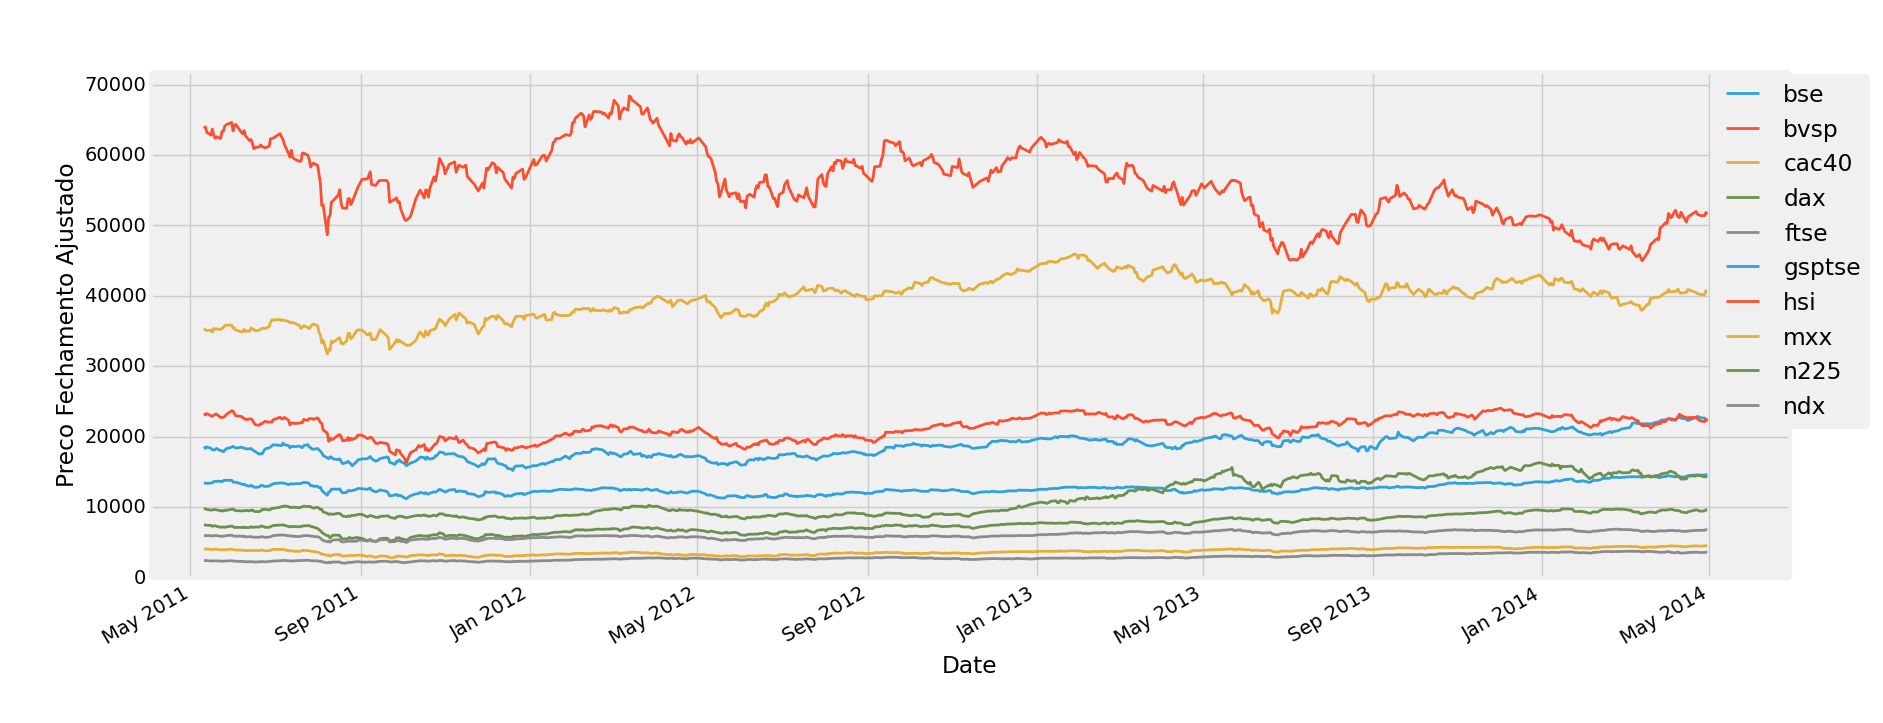
\includegraphics[width=\textwidth]{stocks.png}
            % \caption{Preços de todo o período do conjunto de dados e de todos os índices.}
            % \label{fig:stocks}
            % \end{figure}

            Assim, na Figura~\ref{fig:corr} é mostrada a correlação entre os índices, indicando que o índice GSPTSE é o índice com maior correlação com o índice Bovespa. As maiores correlações com o índice Bovespa são apresentadas pelos índices da américa, sendo que os índices asiáticos apresentam uma correlação menor. Conforme esperado, a correlação é maior entre bolsas de um mesmo continente.

            \begin{figure}[htb]
            \centering
            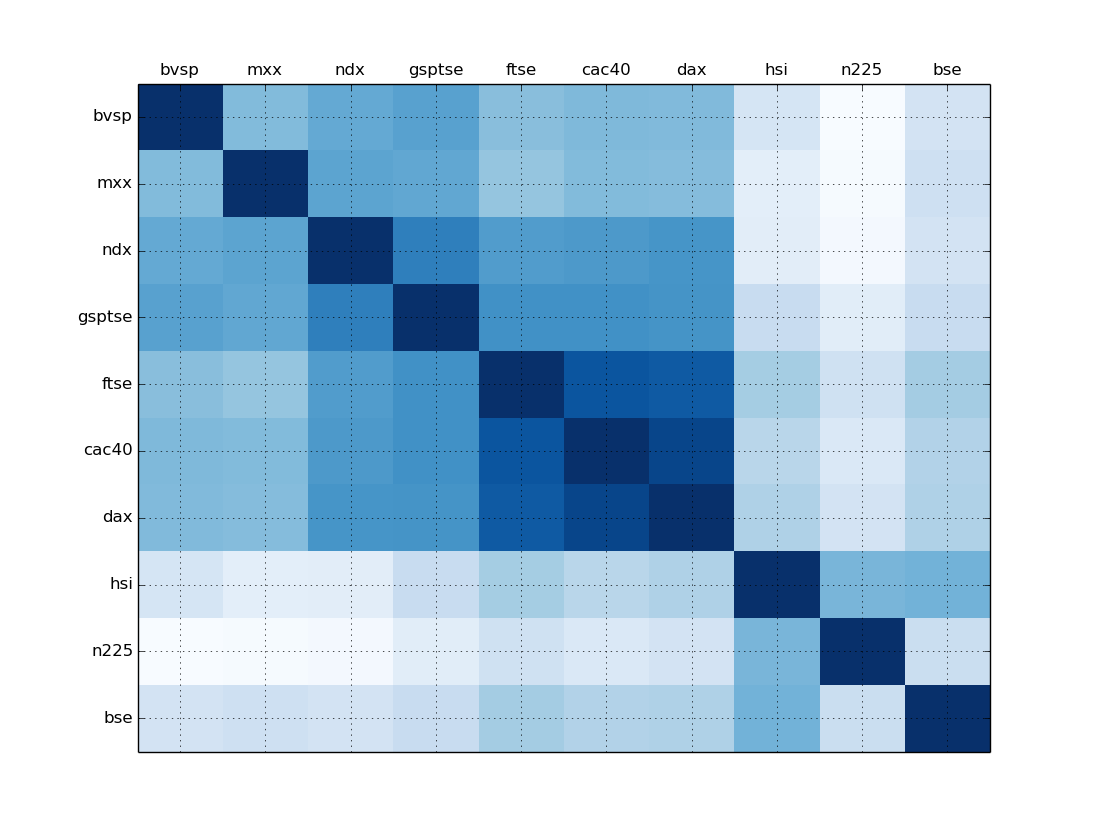
\includegraphics[width=12cm]{correlacao.png}
            \caption{Correlação entre todos os índices usando o período inteiro do conjunto de dados, sendo azul escuro uma correlação maior e azul claro uma correlação menor.}
            \label{fig:corr}
            \end{figure}

        Para analisar o parâmetro janela, foi feita uma autocorrelação do preço de fechamento do índice Bovespa, considerando uma janela de até 30 dias, apresentado na Figura~\ref{fig:autocorr}. É possível ver que não seria adequado estudar o uso de janelas maiores que 10 dias, assim, janelas de até 5 dias foram consideradas.

            \begin{figure}[H]
            \centering
            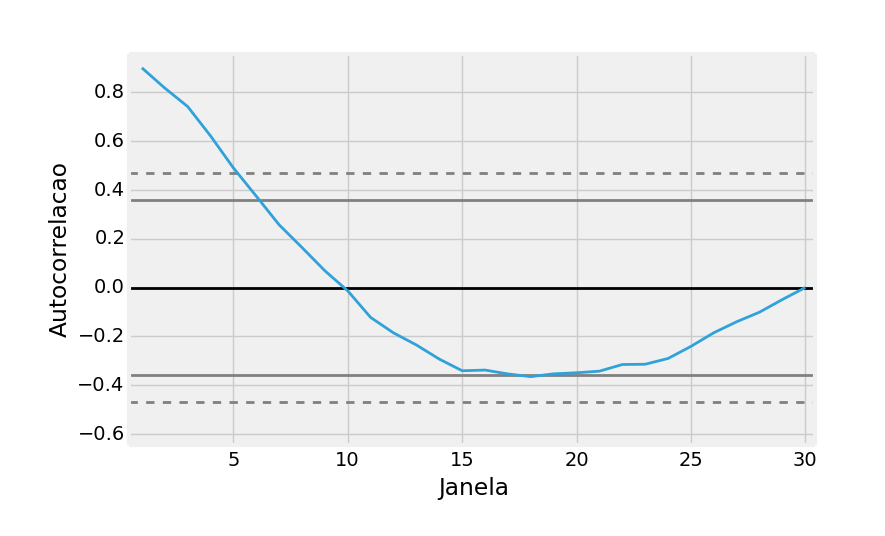
\includegraphics[width=12cm]{autocorrelacao.png}
            \caption{Autocorrelação do índice Bovespa considerando uma janela de até 30 dias.}
            \label{fig:autocorr}
            \end{figure}

        Para realizar a previsão de tendências, quatro métodos de classificação são investigados neste trabalho: Regressão Logística, Redes Neurais Artificiais (\textit{Multilayer Perceptron} -- MLP), as Máquinas de Aprendizado Extremo (\textit{Extreme Machine Learning} -- ELM) e Máquinas de Vetores Suporte (\textit{Support Vector Machines} -- SVM). Esta seção apresenta os resultados para a previsão de tendência do índice Bovespa com cada uma das técnicas, usando a validação cruzada (\textit{Cross-Validation} -- CV) com cinco partições.

        \subsection{Previsão usando Regressão Logística}

        Na Regressão Logística implementada para este trabalho, apenas três parâmetros são considerados: taxa de aprendizado, número máximo de épocas e parâmetro de regularização. Testes preliminares indicaram que 2000 épocas são suficientes para atingir o erro mínimo possível usando gradiente descendente. Portanto, em relação aos parâmetros da regressão logística, variou-se apenas a taxa de aprendizado (0,1; 0,3; 0,5; 0,7; e 0,9) e o parâmetro da regularização (0,001 e 0,01).

            Além disso, como nos demais conjuntos de experimentos, foram analisadas: o uso de uma, duas ou três bolsas por continente, além do uso apenas do índice Bovespa; as combinações de bolsas possíveis; horizonte de previsão de 1, 2, 5 e 20 dias; e janelas de 1 a 5 dias.

        Como a Regressão Logística originalmente foi criada para tratar problemas binários, a estratégia um contra todos foi utilizada para realizar a classificação multiclasse. Nesta estratégia, um classificador binário é criado para cada classe do problema, visando classificar se o dado pertence àquela classe ou não. Cada dado é submetido aos três classificadores e a classe correspondente ao classificador que apresentar a maior saída é escolhida como a classe correspondente àquele dado. \cite{Rifkin2004} mostra que o esquema um contra todos apresenta um bom desempenho comparado às demais estratégias para classificação multiclasse, contanto que use bons classificadores binários.

        Para realizar os testes, foi utilizada a técnica CV com 5 partições usando 80\% dos dados disponíveis. O erro na validação foi considerado para analisar os parâmetros, porém, para obter o resultado para os testes, um novo modelo foi treinado com todos os dados usados no CV, com teste aplicado aos 20\% restantes dos dados. Infelizmente, a variância do CV obtida nos testes mostrou que o algoritmo não se comporta de forma estável para o conjunto de dados utilizado, de forma que os melhores parâmetros obtidos na validação não correspondem necessariamente aos parâmetros que obtém melhores resultados nos testes. Para considerar a variância na escolha dos melhores modelos, calculamos uma estimativa pessimista do erro verdadeiro, a partir do limite superior aproximando a distribuição do erro de uma normal com intervalo de confiança de 95\% sobre o resultado do CV. A seleção dos parâmetros é feita a partir do modelo com melhor estimativa pessimista, calculada a partir do erro médio e do desvio padrão no conjunto de validação. %(erro médio somado a 1,96 multiplicado pelo desvio padrão). A seleção dos parâmetros é feita a partir do modelo com melhor estimativa pessimista, calculada a partir do erro médio e do desvio padrão no conjunto de validação.

        A Regressão Logística é um modelo linear para classificação de padrões. Sendo assim, espera-se que seu desempenho seja reduzido para problemas complexos, cujos elementos de diferentes classes não possam ser classificados por uma superfície de separação linear. De fato, a regressão logística apresenta resultados insatisfatórios para a previsão de tendências do índice Bovespa.

        Considerando apenas o índice Bovespa, o erro médio obtido no CV considerando todas as combinações de parâmetros possíveis foi de 59,31\%. Considerando a melhor estimativa pessimista explicada no parágrafo anterior, o erro de validação obtido foi de 56,5\% e foi apresentado por um modelo com cinco dias na janela, horizonte de previsão de 5 dias, taxa de aprendizado de 0,1 e parâmetro de regularização igual a 0,001. Entretanto, o erro do CV apresentou desvio padrão de 4,6\%, e o erro obtido para o conjunto de testes foi de 65,04\%.

        Usando todas as bolsas de todos os continentes, o erro médio obtido no CV considerando todas as combinações de parâmetros possíveis foi de 59,29\%. Os resultados para a melhor estimativa pessimista são extremamente parecidos com os obtidos usando apenas o ibovespa: 56,5\% de erro médio na validação com um modelo com cinco dias na janela, horizonte de previsão de 5 dias, taxa de aprendizado de 0,1 e parâmetro de regularização igual a 0,001. O erro do CV apresentou desvio padrão de 4,6\%, com erro no teste de 65,04\%.

        No caso da regressão logística aplicada à este problema, nota-se que os parâmetros de taxa de aprendizado e regularização estudados não causam impacto no desempenho aos modelos: fixados os outros parâmetros, os modelos gerados apresentam erros médios de validação similares. Em relação aos demais parâmetros estudados, sob o ponto de vista da aplicação (horizonte de previsão, tamanho de janela, número de bolsas por continente e índices utilizados), apenas o horizonte de previsão parece ter impacto significativo no desempenho do modelo \footnote{A técnica \textit{t-test} foi utilizada considerando a média, desvio padrão e número de experimentos considerado para avaliar se cada par de parâmetro apresentava comportamento diferente de forma estatisticamente significativa. Tais testes consideravam como hipótese nula que não havia diferença entre as médias de erro ao considerar diferentes valores para um mesmo parâmetro. A hipótese nula foi rejeitada -- ou seja, a diferença entre as médias foi considerada significativa -- sempre que o \textit{p-value} obtido foi menor que 0,05.}.

        Dentre os modelos treinados apenas com dados do índice Bovespa, a melhor estimativa pessimista é obtida por um modelo não regularizado que considera horizonte de previsão de 5 dias, janela de cinco dias e taxa de aprendizado igual a 0,1. O erro médio de validação foi de 48,98\%, com desvio padrão de 7,32\%, porém o erro no conjunto de testes foi de 65,04\%. O modelo com melhor desempenho no conjunto de teste obteve 39,5\% de erro, com erro médio de validação de 41,5\% e desvio padrão de 16,3\%. Na média, modelos usando apenas o índice Bovespa apresentaram 51,5\% de erro e desvio padrão de 6,7\%.

        Analisando uma bolsa por continente, a melhor estimativa pessimista é obtida por um modelo não regularizado que considera horizonte de previsão de 5 dias, janela de cinco dias, taxa de aprendizado igual a 0,5 e dados dos índices DAX, GSPTSE e HSI. O erro médio de validação foi de 50,6\%, com desvio padrão de 1,69\%, e o erro no conjunto de testes foi de 65,04\%. Destaca-se que, neste caso, o modelo com melhor desempenho no conjunto de teste (não regularizado com horizonte de previsão de 20 dias, janela de cinco dias, taxa de aprendizado igual a 0,1 e dados dos índices FTSE, GSPTSE e BSE) obteve apenas 8,47\% de erro, porém não foi selecionado devido à alta variância no CV (erro médio de validação de 50,6\% e desvio padrão de 14,6\%). Na média, modelos usando uma bolsa por continente apresentaram 55,5\% de erro e desvio padrão de 6,3\%.

            Analisando duas bolsas por continente, a melhor estimativa pessimista é obtida por um modelo não regularizado que considera horizonte de previsão de 20 dias, janela de quatro dias, taxa de aprendizado igual a 0,9 e dados dos índices CAC 40, DAX, NDX, MXX, BSE e HSI. O erro médio de validação foi de 39,03\%, com desvio padrão de 6,59\%, porém o erro no conjunto de testes foi extremamente alto (96,64\%), com o modelo gerado no teste errando quase todas as instâncias. O modelo com melhor desempenho no conjunto de teste, em compensação, obteve apenas 13,45\% de erro, porém não foi selecionado devido à alta variância no CV (erro médio de validação de 48,1\% e desvio padrão de 10,6\%). Na média, modelos usando duas bolsas por continente apresentaram 57,7\% de erro e desvio padrão de 6,7\%.

            Considerando dados de todos os índices, a melhor estimativa pessimista é obtida por um modelo com parâmetro de regularização igual a 0,01 com horizonte de previsão de 5 dias, janela de cinco dias e taxa de aprendizado igual a 0,3. O erro médio de validação foi de 50,8\%, com desvio padrão de 1,32\%, e o erro no conjunto de testes foi de 65,04\%. O modelo com melhor desempenho no conjunto de teste obteve 21,8\% de erro, com erro médio de validação de 47,2\% e desvio padrão de 12,48\%. Na média, modelos usando todos os índices apresentaram 59,8\% de erro e desvio padrão de 7,2\%.
						
            A partir dos resultados analisados, é possível perceber que, apesar de apresentar resultados surpreendentemente bons em casos específicos, a regressão logística não é uma técnica robusta para resolver o problema, mostrando-se instável e apresentando variância acima da média na validação cruzada.

        %Considerando os resultados apresentados nesta seção, é possível perceber que a variável de maior impacto para o bom desempenho da previsão de tendências do índice Bovespa é o horizonte de previsão. Possivelmente, isso se deve ao fato de que o índice apresenta pequenas oscilações a curto prazo que são difíceis de prever e que não necessariamente representam a tendência do índice naquele dia (visto que avaliamos apenas o valor de fechamento do índice). Além disso, a longo prazo (com o horizonte de previsão de 20 dias) é mais difícil que haja um dado da classe estável (menos de 5\% dos dados no caso da Tabela~\ref{tab:confusao-log}), de forma que o conjunto de classificadores considera que nenhum dado pertence a essa classe (o que causa um erro baixo devido a quantidade de exemplos dessa classe) e existem mais exemplos das classes alta e baixa, o que pode melhorar a classificação destas.

    \subsection{Previsão usando \textit{Multilayer Perceptron}}

        Na MLP implementada, foram considerados os seguintes parâmetros para geração de modelos: número de neurônios na camada escondida (25, 50, 100, 200) e taxa de regularização (0; 0,1; 0,001). Outros parâmetros, como: taxa de aprendizado, taxa de decaimento e acréscimo, número máximo de épocas e \textit{momentum} foram fixados seguindo direções em \cite{haykin2009neural,SutskeverMartensDahlHinton_icml2013,lecun-efficient-backprop-1998,moreira-techrep}. Testes preliminares indicaram que 2000 épocas são suficientes para atingir o erro mínimo possível usando o \textit{backpropagation} modificado. Os parâmetros fixados foram \textit{momentum} máximo 0,99; taxa adaptativa para 0,01; acréscimo da taxa adaptativa 1,05; e decréscimo da taxa adaptativa 0,7.

        Diferentemente da Regressão Logística, a MLP é capaz de lidar com problemas multiclasse, não necessitando de estratégias como um contra todos ou um contra um. Além disso, espera-se que a MLP tenha uma erro de classificação menor que o da Regressão Logística, por ser um modelo que aprende superfícies de decisão complexas e não lineares.

       Neste caso, a estratégia de teste utilizada foi um pouco diferente da usada para regressão logística. Um CV com cinco partições foi usado da mesma forma para validação e seleção de parâmetros (80\% do conjunto de dados disponível), porém o modelo com melhor resultado na validação foi aplicado diretamente aos dados de teste (20\% do conjunto), sem realizar novamente o treinamento com todos os dados disponíveis para validação. A escolha dos parâmetros foi realizada com base na melhor estimativa pessimista.

            Dentre os modelos treinados apenas com dados do índice Bovespa, a melhor estimativa pessimista é obtida por um modelo não regularizado que considera horizonte de previsão de 20 dias, janela de quatro dias e 25 neurônios na camada escondida. O erro médio de validação foi de 32,62\%, com desvio padrão de 5,11\%, porém o erro no conjunto de testes foi de 57,6\% (bem superior ao estimado). O modelo com melhor desempenho no conjunto de teste obteve 10,2\% de erro, com erro médio de validação de 39,26\% e desvio padrão de 4,52\%. Na média, modelos usando apenas o índice Bovespa apresentaram 49,7\% de erro e desvio padrão de 8,8\%.

        Analisando uma bolsa por continente, a melhor estimativa pessimista é obtida por um modelo não regularizado que considera horizonte de previsão de 20 dias, janela de cinco dias, 200 neurônios na camada escondida e dados dos índices DAX, NDX e BSE. O erro médio de validação foi de 26,98\%, com desvio padrão de 4,52\%, e o erro no conjunto de testes foi de 26,3\%. O modelo com melhor desempenho no conjunto de teste obteve 25,4\% de erro, com erro médio de validação de 34,98\% e desvio padrão de 10,78\%. Na média, modelos usando uma bolsa por continente apresentaram 53,1\% de erro e desvio padrão de 9,3\%.

            Analisando duas bolsas por continente, a melhor estimativa pessimista é obtida por um modelo que considera horizonte de previsão de 20 dias, janela de dois dias, 25 neurônios na camada escondida e dados dos índices DAX, FTSE, GSPTSE, MXX, N225 e HSI. O erro médio de validação foi de 22,28\%, com desvio padrão de 6,56\%, porém o erro no conjunto de testes foi maior do que o esperado, de 59,7\%. O modelo com melhor desempenho no conjunto de teste obteve 15,1\% de erro, com erro médio de validação de 33,8\% e desvio padrão de 16,2\%. Na média, modelos usando duas bolsas por continente apresentaram 49,5\% de erro e desvio padrão de 12,2\%.

            Considerando dados de todos os índices, a melhor estimativa pessimista é obtida por um modelo com parâmetro de regularização igual a 0,01 com horizonte de previsão de 20 dias, janela de três dias e 200 neurônios na camada escondida. O erro médio de validação foi de 27,32\%, com desvio padrão de 5,36\%, e o erro no conjunto de testes foi de 34,7\%. O modelo com melhor desempenho no conjunto de teste obteve 12,7\% de erro, com erro médio de validação de 33,04\% e desvio padrão de 12,24\%. Na média, modelos usando três bolsas por continente apresentaram 50,8\% de erro e desvio padrão de 10,9\%.
						
						Para analisar o desempenho da MLP no problema, selecionou-se o modelo obtido para uma bolsa por continente (por apresentar resultados similares na validação e no teste). A Tabela~\ref{tab:confusao-mlp} apresenta as matrizes de confusão para o conjunto de validação e para o conjunto de teste no modelo selecionado usando uma bolsa por continente. 

    \begin{table}[htb]
    \caption{Matriz de confusão do modelo selecionado usando MLP, considerando erros no conjunto de teste.}
    \label{tab:confusao-mlp}
    \centering
    \begin{tabular}{|ccccc|c|ccccc|}
		\cline{1-5} \cline{7-11}
		\multicolumn{5}{|c|}{\textbf{Validação}} & & \multicolumn{5}{|c|}{\textbf{Teste}} \\ 
		\cline{1-5} \cline{7-11}
                      &   & \multicolumn{3}{c|}{Classe Predita} & & &  & \multicolumn{3}{c|}{Classe Predita} \\
               &   & Alta  & Estável   & Baixa & &   & & Alta  & Estável   & Baixa    \\
Classe & Alta & \textbf{38}    & 0     & 16 & 	&			Classe   & Alta & \textbf{34}    & 0     & 5\\
Real   & Estável & 0   & \textbf{0}    & 4 & 		&			Real& Estável & 2   & \textbf{0}    & 2   \\
                                & Baixa & 0    & 0 & \textbf{36}   & && Baixa & 22    & 0 & \textbf{53}  \\
\cline{1-5} \cline{7-11}
    \end{tabular}
    \end{table}
		
		A partir dos resultados, é possível observar que a classe estável apresenta poucas instâncias, tanto no conjunto de validação quanto no conjunto de testes. Isso ocorre porque, ao usar um horizonte de previsão de 20 dias, é difícil que o preço da ação não mude pelo menos 0,5\%. Sendo assim, ao usar esse horizonte de previsão, o problema praticamente se reduz a um problema binário, apresentando erros menores. Analisando apenas as classes alta e baixa, é possível perceber que ainda há razoável confusão entre as classes: no conjunto de teste, a classe alta apresenta 91\% de revocação, mas apenas 59\% de precisão; na validação, 70\% de revocação e 64\% de precisão. 
						
            Em relação aos parâmetros da MLP, foi possível notar que os parâmetros de regularização usados não influenciaram nos modelos gerados, visto que modelos idênticos foram gerados com diferentes fatores de regularização. Em relação ao número de neurônios, percebe-se que, ao usar uma bolsa por continente, quanto maior o número de neurônios, menor o erro obtido pelo modelo. Nos demais testes, o número de neurônios não se mostrou como um parâmetro importante para o resultado. Como trabalho futuro, seria interessante estudar o uso de redes neurais com número de neurônios superior a 200 para o problema.

            Em relação aos parâmetros da aplicação, é interessante notar que, ao considerar uma bolsa por continente com a MLP, o tamanho da janela parece ter uma pequena influência nos resultados: modelos que usam janelas maiores (entre três e cinco dias) apresentam uma média de erro um pouco inferior (porém estatisticamente significativa) aos que usam dados não janelados. Ao usar todos os índices ou apenas o índice Bovespa, o tamanho da janela não influencia significativamente nos resultados. Em relação aos índices considerados, é interessante notar que o índice HSI, que está associado a bons resultados usando a outras técnicas, não é tão importante ao usar a MLP com uma bolsa por continente.

        \subsection{Previsão usando \textit{Extreme Learning Machines}}

        Neste trabalho, \textit{Extreme Learning Machines} (ELM) foram utilizadas considerando os seguintes parâmetros: número de neurônios (100, 300, 500, 700 e 900) e um parâmetro de regularização (0,001 e 0,01). Não foi utilizada a ELM sem regularização porque, neste problema, a matriz $H$ necessita do processo de regularização para se tornar invertível.

        A estratégia de teste utilizada foi a mesma usada para regressão logística: CV com cinco partições para validação e seleção de parâmetros (80\% do conjunto de dados disponível), com a construção de um novo modelo treinado com todos os dados da validação para ser aplicado aos dados de teste (20\% do conjunto). A escolha dos parâmetros também foi realizada com base na melhor estimativa pessimista, descrita anteriormente.

        Considerando apenas o índice Bovespa, o erro médio obtido no CV considerando todas as combinações de parâmetros possíveis foi de 51,3\% . Considerando a melhor estimativa pessimista explicada no parágrafo anterior, o erro de validação obtido foi de 44,24\% e foi apresentado por um modelo com apenas um dado na janela, horizonte de previsão de 5 dias, 300 neurônios na camada escondida e parâmetro de regularização igual a 0,01. Entretanto, o erro do CV apresentou desvio padrão considerável, de 5,8\%, e o erro obtido para o conjunto de testes foi mais alto que o esperado (65,32\%).

        No outro extremo, usando todas as bolsas de todos os continentes, o erro médio obtido no CV considerando todas as combinações de parâmetros possíveis foi de 54,7\% e desvio padrão de 7,8\%. Já a melhor estimativa pessimista neste caso apresentou 51,63\% de erro médio na validação e foi apresentado por um modelo com cinco dados na janela, horizonte de previsão de 5 dias, 700 neurônios na camada escondida e parâmetro de regularização igual a 0,01. Desta vez, o erro do CV apresentou desvio padrão baixo, de 1,7\%, com erro no teste de 54,47\% (dentro do esperado segundo a estimativa). Dentre os cinco modelos com melhores estimativas pessimistas, foram obtidos erros de teste mais baixos, de até 43,55\%.

        Já usando apenas uma bolsa por continente, o erro médio obtido no CV considerando todas as combinações de parâmetros possíveis foi de 53,46\% e desvio padrão de 9,3\%. Já o erro de validação obtido com a melhor estimativa pessimista foi de 34,24\% e foi apresentado por um modelo com dois dados na janela, horizonte de previsão de 20 dias, 900 neurônios na camada escondida e parâmetro de regularização igual a 0,01. Os índices considerados neste modelo foram os índices FTSE, MXX e HSI. O erro do CV apresentou desvio padrão razoável, de 7,4\%, e o erro obtido para o conjunto de testes foi de 34,45\%, muito próximo ao erro de validação.

        Usando duas bolsas por continente, o erro médio obtido no CV considerando todas as combinações de parâmetros possíveis foi de 54,06\%  e desvio padrão de 8,1\%. O erro de validação obtido com a melhor estimativa pessimista foi de 40,34\% e foi apresentado por um modelo com dois dados na janela, horizonte de previsão de 20 dias, 100 neurônios na camada escondida e parâmetro de regularização igual a 0,01. Os índices considerados foram CAC 40, FTSE, NDX, GSPTSE, BSE e HSI. O erro do CV apresentou desvio padrão razoável, de 4,09\%, e o erro obtido para o conjunto de testes foi de 40,34\%, dentro do esperado a partir do erro médio de validação.

        Para todos os casos, resultados melhores foram obtidos tanto para validação quanto para teste. Os melhores resultados na validação, porém, apresentaram alta variância e resultados ruins no teste. Para exemplificar a dificuldade em estimar um modelo usando CV para esse problema, foi possível encontrar um erro mínimo de 14,29\% para o conjunto de testes com duas bolsas por continente, porém tal modelo apresentou erro médio de 38,03\% no CV e desvio padrão de 14,37\%, de forma a não figurar entre as melhores estimativas pessimistas ou os menores erros médios no CV. Comparativamente, o menor erro de validação foi de 28,03\%, com uma bolsa por continente, mas apresentou desvio padrão de 10,45\% e erro no teste de 66,39\%, bem maior que o esperado.

        Também foram realizadas análises para avaliar o impacto de cada parâmetro no modelo. Tais análises foram realizadas separadamente para cada caso (apenas ibovespa, uma bolsa por continente, duas bolsas por continente e três bolsas por continente). Em todos os casos, dentre janela, horizonte de previsão, número de neurônios e parâmetro de regularização, apenas o horizonte de previsão apresentou um impacto estatisticamente significativo na média dos erros de validação obtidos. Os gráficos da Figura~\ref{fig:elm-horizonte} apresentam a média dos erros na validação para cada caso, investigado de acordo com o horizonte de previsão.

     \begin{figure}[htb]
     \centering
     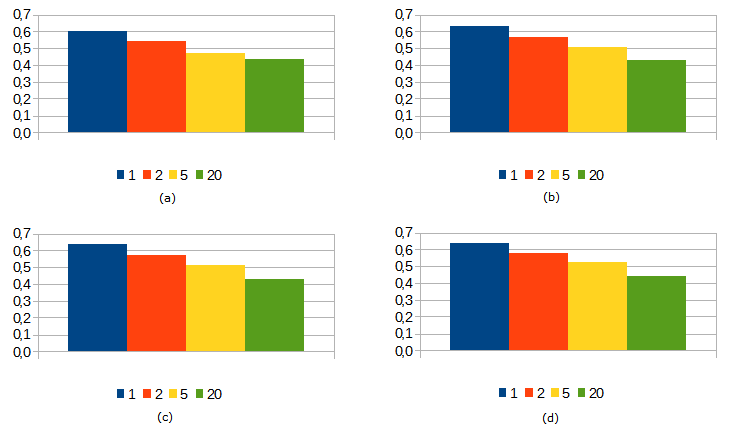
\includegraphics[width=\textwidth]{elm-horizonte.png}
     \caption{Erro médio por horizonte de previsão, considerando: (a) apenas a ibovespa; (b) uma bolsa por continente; (c) duas bolsas por continente; (d) três bolsas por continente. }
     \label{fig:elm-horizonte}
     \end{figure}
  

        Em relação aos índices utilizados, os resultados indicam que alguns índices colaboram mais para melhores resultados. Dentre os índices da Ásia, o índice HSI parece favorecer melhores resultados, visto que aparece nas melhores combinações de índices tanto quando consideramos apenas uma bolsa por continente (4 das 5 melhores médias), quanto quando consideramos duas bolsas por continente (5 das 5 melhores médias). Em menor grau, os índices CAC 40 (3 das 5 melhores médias com uma bolsa e 5 das 5 melhores médias com duas bolsas) e NDX aparecem com maior frequência nas melhores combinações (2 das 5 melhores médias com uma bolsa e 4 das 5 melhores médias com duas bolsas). Porém é importante notar que não existe diferença significativa entre as cinco melhores médias em relação às combinações de índices utilizados. A Tabela~\ref{tab:elm-ind} apresenta a média e desvio padrão obtido a partir dos resultados dos experimentos usando cada uma das combinações de índices possível, com uma ou duas bolsas por continente.


    \begin{table}[htb]
    \caption{Erro médio e desvio padrão para cada combinação de índices possível usando uma ou duas bolsas por continente. Os números correspondem ao índice utilizado, sendo: (1) CAC 40; (2) DAX; (3) FTSE; (4) NDX; (5) GSPTSE; (6) MXX; (7) N225; (8) BSE; (9) HSI.}
    \label{tab:elm-ind}
		\footnotesize
    \centering
    \begin{tabular}{|ccc||ccc|}
    \hline
    \multicolumn{3}{|c||}{\textbf{Uma bolsa por continente}} & \multicolumn{3}{|c|}{\textbf{Duas bolsas por continente}} \\
    \hline  Índices &Erro médio  &  Desvio Padrão  & Índices &Erro médio  &  Desvio Padrão\\
    \hline
    2-6-9   &   0,5229  &   0,0820  &   1-4-9-2-6-8 &   0,5260  &   0,0846  \\
    1-5-9   &   0,5255  &   0,0800  &   1-4-9-2-5-8 &   0,5288  &   0,0783  \\
    1-5-7   &   0,5258  &   0,0936  &   1-5-9-2-6-8 &   0,5293  &   0,0871  \\
    2-4-9   &   0,5261  &   0,0786  &   1-4-9-3-5-8 &   0,5299  &   0,0852  \\
    1-4-9   &   0,5273  &   0,0839  &   1-4-9-3-6-8 &   0,5303  &   0,0872  \\
    3-4-9   &   0,5277  &   0,0808  &   2-4-9-3-6-8 &   0,5303  &   0,0837  \\
    2-5-9   &   0,5287  &   0,0774  &   1-5-9-3-6-8 &   0,5326  &   0,0851  \\
    1-5-8   &   0,5288  &   0,0755  &   2-5-9-3-6-8 &   0,5333  &   0,0828  \\
    1-6-9   &   0,5300  &   0,0789  &   2-4-9-3-5-8 &   0,5362  &   0,0743  \\
    2-5-7   &   0,5308  &   0,0862  &   1-4-7-3-5-8 &   0,5369  &   0,0952  \\
    3-5-9   &   0,5318  &   0,0789  &   2-4-7-3-5-9 &   0,5379  &   0,0854  \\
    3-6-9   &   0,5330  &   0,0780  &   1-4-7-3-5-9 &   0,5385  &   0,0932  \\
    2-4-7   &   0,5333  &   0,0803  &   2-4-7-3-5-8 &   0,5387  &   0,0856  \\
    1-4-7   &   0,5345  &   0,0948  &   1-4-7-2-5-8 &   0,5390  &   0,0876  \\
    3-5-7   &   0,5350  &   0,0845  &   1-4-7-2-5-9 &   0,5404  &   0,0868  \\
    2-5-8   &   0,5351  &   0,0708  &   2-4-7-3-6-8 &   0,5452  &   0,0732  \\
    2-6-8   &   0,5351  &   0,0783  &   1-4-7-2-6-9 &   0,5455  &   0,0786  \\
    1-4-8   &   0,5361  &   0,0817  &   2-5-7-3-6-9 &   0,5477  &   0,0744  \\
    2-4-8   &   0,5381  &   0,0695  &   2-4-7-3-6-9 &   0,5480  &   0,0721  \\
    2-6-7   &   0,5398  &   0,0665  &   1-5-7-2-6-8 &   0,5481  &   0,0766  \\
    3-5-8   &   0,5404  &   0,0704  &   1-5-7-2-6-9 &   0,5483  &   0,0737  \\
    3-4-8   &   0,5407  &   0,0714  &   1-4-7-2-6-8 &   0,5490  &   0,0749  \\
    3-4-7   &   0,5419  &   0,0769  &   2-5-7-3-6-8 &   0,5492  &   0,0749  \\
    1-6-8   &   0,5423  &   0,0753  &   1-4-7-3-6-8 &   0,5500  &   0,0765  \\
    3-6-8   &   0,5457  &   0,0712  &   1-4-7-3-6-9 &   0,5518  &   0,0754  \\
    1-6-7   &   0,5483  &   0,0687  &   1-5-7-3-6-8 &   0,5523  &   0,0762  \\
    3-6-7   &   0,5501  &   0,0622  &   1-5-7-3-6-9 &   0,5525  &   0,0768  \\

    \hline
    \end{tabular}
    \end{table}

    Em resumo, o melhor modelo ao considerar a estimativa pessimista do erro verdadeiro foi obtido com uma bolsa por continente, apresentando erro de validação de 34,24\% e erro no teste de 34,45\%. Os parâmetros usados foram: janela de dois dias, horizonte de previsão de 20 dias, 900 neurônios na camada escondida e parâmetro de regularização igual a 0,01. A Tabela~\ref{tab:confusao-elm} apresenta a matriz de confusão para o conjunto de teste. Novamente, assim como visto para a MLP, existe razoável confusão entre as classes alta e baixa, mostrando que as técnicas utilizadas apresentam dificuldades para distinguir as classes do problema estudado.

    \begin{table}[htb]
    \caption{Matriz de confusão do modelo selecionado usando ELM, considerando erros no conjunto de teste.}
    \label{tab:confusao-elm}
    \centering
    \begin{tabular}{cccccc}
                                &   & \multicolumn{3}{c}{Classe Predita} \\
                                &   & Alta  & Estável   & Baixa     \\
    \multirow{3}{*}{Classe Real}& Alta & \textbf{33}    & 0     & 7 \\
                                & Estável & 2   & \textbf{0}    & 2     \\
                                & Baixa & 30    & 0 & \textbf{45}       \\

    \end{tabular}
    \end{table}


    \subsection{Previsão usando \textit{Support Vector Machines}}

        Neste trabalho, \textit{Support Vector Machines} (SVM) foram utilizadas variando apenas o parâmetro de margem (C). Foi utilizado o kernel linear e, portanto, não há parâmetros associados ao kernel. A SVM, assim como a regressão logística, foi desenvolvida para problemas binários. Portanto, a estratégia um contra todos também foi usada com a SVM para aplicar a técnica ao problema multiclasse.

        A estratégia de teste utilizada foi a mesma usada para MLP: CV com cinco partições para validação e seleção de parâmetros (80\% do conjunto de dados disponível), usando o modelo com melhor resultado na validação para ser aplicado aos dados de teste (20\% do conjunto). Assim como para todas as demais técnicas, a escolha dos parâmetros também foi realizada com base na melhor estimativa pessimista.

        Para uma bolsa por continente, a melhor estimativa pessimista foi obtida por um modelo com $C=1$, horizonte de previsão de 20 dias e janela de dois dias, considerando os índices DAX, NDX e BSE. O erro médio na validação foi de 30,88\%, com 1,46\% de desvio padrão, apresentando 35,3\% de erro no conjunto de teste. No conjunto de teste, o menor erro obtido foi de 9,3\% (erro médio no CV de 37,04\% e desvio padrão de 12,49\%).

        Para duas bolsas por continente, a melhor estimativa pessimista foi obtida por um modelo com $C=1$, horizonte de previsão de 20 dias e janela de um dia, considerando os índices DAX, FTSE, NDX, GSPTSE, BSE e HSI. O erro médio na validação foi de 30,18\%, com 3,21\% de desvio padrão. Porém, o erro no conjunto de teste foi muito superior ao estimado (62,2\%). Dentre os cinco modelos com melhores estimativas pessimistas, foi encontrado um modelo cujo erro no conjunto de teste foi de apenas 16\% e, dentre todos os modelos gerados para duas bolsas por continente, foi possível encontrar modelos com apenas 11,9\% de erro no teste.

        Considerando todos os índices, a melhor estimativa pessimista foi obtida por um modelo com $C=10$, horizonte de previsão de 5 dias e janela de 4 dias. O erro médio na validação foi de 53,34\%, com 2,59\% de desvio padrão. No conjunto de testes, o erro obtido 43,1\%. No melhor caso, o erro no conjunto de testes foi de 14,3\% (erro médio no CV de 32,8\% e desvio padrão de 14,06\%).

        Se considerarmos apenas o índice Bovespa, por outro lado, a melhor estimativa pessimista foi obtida por um modelo com $C=100$, horizonte de previsão de 20 dias e janela de 5 dias, atingindo um erro médio na validação de 35,46\%, com 5,39\% de desvio padrão. No conjunto de testes, porém, o erro obtido foi maior do que o estimado (66,9\%). De qualquer forma, o menor erro obtido no conjunto de testes foi de 56,5\%, indicando que usar apenas o índice Bovespa não é uma boa estratégia para previsão de tendências do índice.

        Uma análise do impacto de cada parâmetro no desempenho dos modelos indica que, na média, parâmetros menores de margem ($C=\{0,01;0,1\}$) estão associados a taxas de erro menores. Em relação aos parâmetros da aplicação, novamente nota-se que a janela não apresenta impacto significativo no desempenho dos modelos, enquanto o horizonte de previsão influencia fortemente o desempenho: quanto maior o horizonte, menor o erro. Novamente, o índice HSI parece ser relevante para minimizar o erro, estando frequentemente associado às combinações de índices que produzem menores médias de erro.
				
				Para ilustrar a dificuldade na seleção de modelos, a Tabela~\ref{tab:confusao-svm} apresenta as matrizes de confusão para os conjuntos de validação e teste considerando o melhor modelo obtido para SVM. Apesar do erro baixo, o modelo obtido considera todas as instâncias do teste como pertencentes à classe baixa. O erro é baixo devido ao desbalanceamento do conjunto, com 63\% das instâncias pertencentes à classe baixa, 34\% pertencentes à classe alta e apenas 3\% pertencentes à classe estável. Para evitar esse problema, outras métricas poderiam ser utilizadas para avaliar e selecionar o modelo, como F-score, uma métrica baseada na revocação e na precisão do modelo.
				
				    \begin{table}[htb]
    \caption{Matriz de confusão do modelo selecionado usando SVM, para os conjuntos de validação e teste}
    \label{tab:confusao-svm}
    \centering
    \begin{tabular}{|ccccc|c|ccccc|}
		\cline{1-5} \cline{7-11}
		\multicolumn{5}{|c|}{\textbf{Validação}} & & \multicolumn{5}{|c|}{\textbf{Teste}} \\ 
		\cline{1-5} \cline{7-11}
                      &   & \multicolumn{3}{c|}{Classe Predita} & & &  & \multicolumn{3}{c|}{Classe Predita} \\
               &   & Alta  & Estável   & Baixa & &   & & Alta  & Estável   & Baixa    \\
Classe & Alta & \textbf{18}    & 0     & 35 & 	&			Classe   & Alta & \textbf{0}    & 0     & 40\\
Real   & Estável & 0   & \textbf{0}    & 4 & 		&			Real& Estável & 0   & \textbf{0}    & 4   \\
                                & Baixa & 0    & 0 & \textbf{38}   & && Baixa & 0    & 0 & \textbf{75}  \\
\cline{1-5} \cline{7-11}
    \end{tabular}
    \end{table}

    \subsection{Discussão dos resultados}

    A partir dos resultados apresentados, é possível perceber que a variável de maior impacto positivo da previsão de tendências do índice Bovespa é o horizonte de previsão. Possivelmente, isso se deve ao fato de que o índice apresenta pequenas oscilações a curto prazo que são difíceis de prever e que não necessariamente representam a tendência do índice naquele dia (visto que avaliamos apenas o valor de fechamento do índice). Além disso, a longo prazo (com o horizonte de previsão de 20 dias) é mais difícil que haja um dado da classe estável, de forma que o conjunto de classificadores considera que nenhum dado pertence a essa classe (o que causa um erro baixo devido a quantidade de exemplos dessa classe) e existem mais exemplos das classes alta e baixa, o que pode melhorar a classificação destas.

    Os resultados indicam que, de forma geral, o tamanho da janela não altera significativamente o desempenho dos modelos.

    Sobre a quantidade de índices/bolsas usados para previsão do índice Bovespa, a média de erros considerando diferentes quantidade indica que o excesso de informação ao usar um grande número de índices poderia confundir o modelo. Porém, ao analisar os melhores resultados, é possível perceber que, de forma geral, os melhores resultados associados a modelos que usam apenas o índice Bovespa são piores que os melhores resultados associados aos demais modelos, indicando que as informações sobre os demais índices podem auxiliar na classificação.

    Em relação aos índices utilizados, destaca-se que, ao usar uma bolsa por continente, a combinação DAX, NDX e BSE fornece os modelos selecionados usando MLP e SVM. Esses índices também aparecem em quase todos os modelos com duas bolsas por continente. O índice HSI também é recorrente, sendo usado em todos os modelos selecionados com duas bolsas por continente. Já o índice N225 é um dos índices que menos frequentes nos modelos com melhores desempenho. Tal fato pode ser explicado devido à baixa correlação entre o índice N225 e o índice Bovespa, como pode ser observado no gráfico de correlação entre índices da Figura~\ref{fig:corr}.
		
		
Para melhor visualização dos melhores resultados obtidos, a Tabela~\ref{tab:sum} apresenta os resultados dos melhores modelos de cada técnica sumarizados agrupados por combinações de bolsas, destacando o melhor modelo obtido ao considerar a estimativa pessimista para seleção de parâmetros: Redes Neurais MLP com 26,3\% de erro no conjunto de teste.

    % \begin{landscape}
    \begin{table}[H]
    \centering
    \caption{Sumarização dos resultados de cada técnica considerando diferentes combinações de bolsas.}
    \label{tab:sum}
    \begin{tabular}{ccccc}
    \hline
                                                                               & \multicolumn{2}{c}{\textbf{Regressão Logística}}                                                                                            & \multicolumn{2}{c}{\textbf{ELM}}                                                                                                            \\ \hline
                                                                               & \textbf{\begin{tabular}[c]{@{}c@{}}Erro\\ Validação (\%)\end{tabular}} & \textbf{\begin{tabular}[c]{@{}c@{}}Erro\\ Teste (\%)\end{tabular}} & \textbf{\begin{tabular}[c]{@{}c@{}}Erro\\ Validação (\%)\end{tabular}} & \textbf{\begin{tabular}[c]{@{}c@{}}Erro\\ Teste (\%)\end{tabular}} \\ \hline
    \textbf{\begin{tabular}[c]{@{}c@{}}1 bolsa por\\  continente\end{tabular}} & $50,6\pm1,69$                                                          & $65,04$                                                            & $34,24\pm7,4$                                                          & $34,45$                                                            \\ \hline
    \textbf{\begin{tabular}[c]{@{}c@{}}2 bolsas\\ por continente\end{tabular}} & $39,03\pm6,59$                                                         & $96,64$                                                            & $40,34\pm4,09$                                                         & $40,34$                                                            \\ \hline
    \textbf{todas as bolsas}                                                   & $50,08\pm1,32$                                                         & $65,04$                                                            & $51,03\pm1,7$                                                          & $54,47$                                                            \\ \hline
    \textbf{IBovespa}                                                          & $48,98\pm7,32$                                                         & $65,04$                                                            & $44,24\pm5,8$                                                          & $65,32$                                                            \\ \hline
    \multicolumn{1}{l}{}                                                       & \multicolumn{2}{c}{\textbf{MLP}}                                                                                                            & \multicolumn{2}{c}{\textbf{SVM}}                                                                                                            \\ \hline
    \multicolumn{1}{l}{}                                                       & \textbf{\begin{tabular}[c]{@{}c@{}}Erro\\ Validação (\%)\end{tabular}} & \textbf{\begin{tabular}[c]{@{}c@{}}Erro\\ Teste (\%)\end{tabular}} & \textbf{\begin{tabular}[c]{@{}c@{}}Erro\\ Validação (\%)\end{tabular}} & \textbf{\begin{tabular}[c]{@{}c@{}}Erro\\ Teste (\%)\end{tabular}} \\ \hline
    \textbf{\begin{tabular}[c]{@{}c@{}}1 bolsa por\\ continente\end{tabular}}  & \textit{$26,98\pm4,52$}                                                & \textit{$26,3$}                                                    & $30,88\pm1,46$                                                         & $35,3$                                                             \\ \hline
    \textbf{\begin{tabular}[c]{@{}c@{}}2 bolsas\\ por continente\end{tabular}} & $22,28\pm4,52$                                                         & $59,7$                                                             & $30,18\pm3,21$                                                         & $62,2$                                                             \\ \hline
    \textbf{todas as bolsas}                                                   & $27,32\pm5,36$                                                         & $34,7$                                                             & $53,34\pm2,59$                                                         & $43,1$                                                             \\ \hline
    \textbf{IBovespa}                                                          & $32,62\pm5,11$                                                         & $57,6$                                                             & $35,46\pm5,39$                                                         & $66,9$                                                             \\ \hline
    \end{tabular}
    \end{table}

É possível notar que os modelos, de forma geral, apresentam alguma instabilidade entre os resultados obtidos para validação e teste, indicando que o problema pode ser complexo para que haja um desempenho estável das técnicas estudadas. É importante lembrar que foram encontrados resultados melhores tanto na validação quanto no teste, porém tais resultados não foram selecionados devido à metodologia de seleção de parâmetros utilizada, que considera não apenas o erro médio no conjunto de validação como também a variância desse erro. Dessa forma, apesar da falta de estabilidade, as técnicas apresentam potencial para atingir resultados melhores.

\section{Conclusão} \label{sec:conclusao}
    Neste trabalho foi feita uma aplicação de técnicas de Aprendizado de Máquina (Regressão Logística, ELM, Redes Neurais MLP e SVM) para prever tendências (alta, baixa e estável) do índice Bovespa, fazendo uma análise de como outros índices do mundo, e parâmetros como janela e horizonte de previsão influenciam na taxa de erro das técnicas aplicadas, fazendo o uso de \textit{Cross-validation} e testes estatísticos.

    Além disso, na fase de seleção dos modelos, considerando os hiperparâmetros de cada modelo, foi possível perceber que modelos regularizados não têm muita influência na predição da tendência do IBovespa. Considerando os parâmetros do problema, é possível afirmar que modelos com horizonte de previsão de 20 dias estão associados à menores taxas de erro e, apesar de estatisticamente a janela não apresentar influência significativa, foi percebido que janelas maiores que 3 dias estão associadas aos melhores modelos.

    Os melhores resultados dos modelos no conjunto de validação mostrou que ao invés de considerar todas as bolsas ou somente o IBovespa para a classificação, os melhores modelos são apresentados considerando 1 ou duas bolsas por continente. Ainda, a combinação de índices DAX, NDX e BSE estão frequentemente presentes nos melhores modelos apresentados. Além destes, o índice HSI (Hong Kong) tem uma influência positiva nas técnicas de Regressão Logística, ELM e SVM, apesar de este apresentar uma correlação menor com o índice Bovespa.

    Analisando os trabalhos correlatos, pode-se dizer que este trabalho obteve uma taxa de erro aceitável usando o modelo de Rede Neural MLP (26,3\% no conjunto de teste). Também é preciso lembrar que resultados melhores foram obtidos tanto nos conjuntos de validação e teste, porém tais resultados não foram selecionados de acordo com a metodologia de seleção de parâmetros utilizada.

    Como trabalhos futuros, seria interessante a realização de mais testes considerando mais variações dos hiperparâmetros de cada modelo, e considerar o uso de estratégias melhores para seleção dos modelos e hiperparâmetros.

% Início da bibliografia
\bibliographystyle{ppgsi}
\bibliography{rt_ep}

% Apêndices
%\appendix
%
%\appsection{Apêndice 1}
    %Texto do apêndice 1
%
%\appsection{Apêndice 2}
    %Texto do apêndice 2

\end{document}
